
%(BEGIN_QUESTION)
% Copyright 2014, Tony R. Kuphaldt, released under the Creative Commons Attribution License (v 1.0)
% This means you may do almost anything with this work of mine, so long as you give me proper credit

Beregn spenningen mellom punkt A og B i denne kretsen, og tegn et fasordiagram som viser hvordan alle spenningene henger sammen:

$$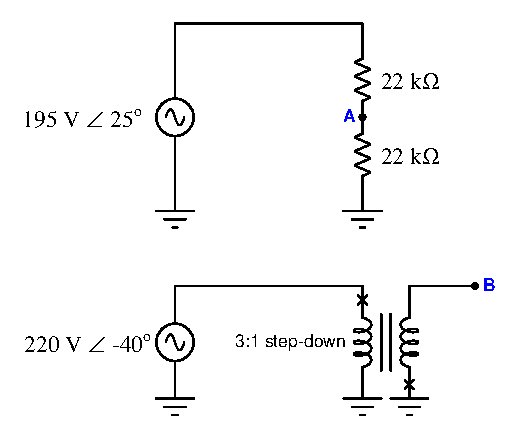
\includegraphics[width=15.5cm]{i00834x01.eps}$$

\underbar{file i00834}
%(END_QUESTION)





%(BEGIN_ANSWER)

Først beregnes spenningene mellom hvert testpunkt og jord. $V_A$ er ganske enkelt første kildespenning delt på 2 i motstandsnettet. $V_B$ er en tredel av kildespenningen, med ekstra faseskift på 180$^{o}$ fra reversert polaritet i sekundærviklingen:

$$V_A = {195 \hbox{ V} \angle 25^o \over 2} = 97.5 \hbox{ V} \angle 25^o$$

$$V_B = {-(220 \hbox{ V} \angle -40^o) \over 3} = 73.33 \hbox{ V} \angle 140^o$$

Når disse to tegnes i et fasordiagram, kan $V_{AB}$ plottes som avstanden mellom $V_A$- og $V_B$-fasorene:

$$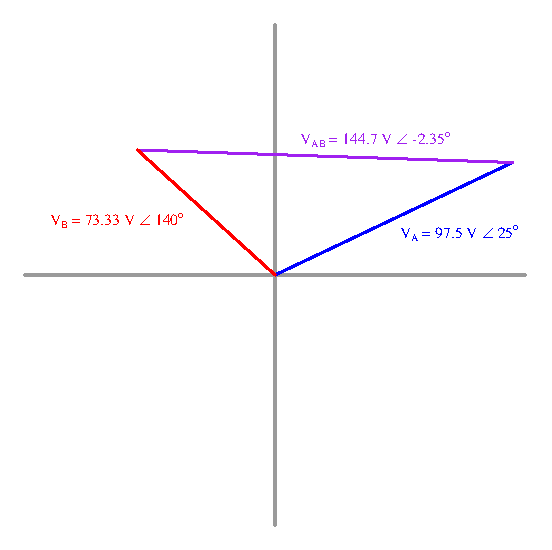
\includegraphics[width=15.5cm]{i00834x02.eps}$$

Spenningen $V_{AB}$ er differansen mellom $V_A$ og $V_B$:

$$V_{AB} = V_A - V_B$$

$$V_{AB} = (97.5 \hbox{ V} \angle 25^o) - (73.33 \hbox{ V} \angle 140^o)$$

$$V_{AB} = 144.7 \hbox{ V} \angle -2.35^o$$

%(END_ANSWER)





%(BEGIN_NOTES)


%INDEX% Electronics review: AC transformer circuit
%INDEX% Electronics review, phasor expressions of circuit quantities

%(END_NOTES)
